\documentclass[11pt, letterpaper]{article}
\usepackage{graphicx}
\usepackage[margin=1in]{geometry}
\usepackage{fancyhdr}
\usepackage[T1]{fontenc}
\usepackage{tabularx}
\usepackage[table, dvipsnames]{xcolor}
\usepackage{amssymb}
\usepackage{tikz}

\let\oldemptyset\emptyset
\let\emptyset\varnothing

\pagestyle{fancy}
\renewcommand{\headrulewidth}{0pt}

\fancyhf{}
\fancyfoot[R]{\thepage}

\begin{document}

\noindent Riley Rice\\CS321\\10-21-2024

\begin{center}\noindent {\Huge \textbf{Homework 2}}\end{center}

\section*{Problem 1: [5 points]}

Suppose $M_1 = (Q_1, \sum, \delta_1, S_1, F_1)$ and $M_2 = (Q_2, \sum, \delta_2, S_2, F_2)$ are two DFAs over the same alphabet. Construct another DFA that decides the language $L(M_1) \setminus  L(M_2)$, i.e., the language consisting of all strings in $L(M_1)$ but not in $L(M_2)$. You must describe the DFA using the formal definition. (This problem is about DFAs only, and has nothing to do with NFAs or $\epsilon$-NFAs.)

\vspace{5mm}

\noindent \textbf{Hint:} Use the theorems in Lec 4, i.e., regular languages are closed under set intersection and complement.

\vspace{5mm}

\noindent\textbf{Solution:}
 
\vspace {5mm}
 
\noindent This new DFA $L(M') = L(M_1) \setminus L(M_2)$, i.e $M'$ is equivalent to:
 
\vspace{5mm}
 
\noindent$Q' = Q_1 \times Q_2$ (Use all the states from both DFAs)\\
$\sum = \sum$ (Uses the same alphabet as $L(M_1)$ and $L(M_2)$)\\
$\delta'((q_1, q_2), c) = (\delta_1(q_1, c), \delta_2(q_2, c))$ (Use both transition functions)\\
$S' = (S_1, S_2)$ (Use both starting states)\\
$F' = \{(q_1, q_2) \in Q' |  q_1 \in F_1$ and $q_2 \notin F_2\}$ (Only accept when the state is accepted in $M_1$ and not $M_2$)\\

\noindent \textbf{Explanation:}

\vspace{5mm}

\noindent In order to come to this I broke down what $L(M_1) \setminus L(M_2)$ means which is equivalent to $L(M_1) \cap \overline{L(M_2)}$. What this means is that we want to find all the strings in $L(M_1)$  that aren't in $L(M_2)$. The good thing about looking at it this way is that we have some theorems for complements and the intersection of DFAs that can be used to create the new DFA and it's a lot easier to apply them in this form. The first thing we want to do is find the complement for $L(M_2)$ which is defined by making $F' = Q \setminus F = \{x \in Q| x \notin F\}$, or in other words accept on all the elements that are in set $Q$ but not in set $F$ which essentially inverts what is accepted for a DFA. You can see that I created the complement of $L(M_2)$ by accepting on states that are accepted by $L(M_1)$ but not accepted by $L(M_2)$ this makes it so the new DFA will only accept on strings that are in $L(M_1)$ but not $L(M_2)$.  Then with the accepting states figured out now we have to get the intersection of $L(M_1)$ and $\overline{L(M_2)}$ which is pretty easy. According to the theorem all we have to do is run the two DFAs in parallel which I do by setting $Q'$ to the cartesian product of the states from both DFAs. I then run both the transition functions and use the two starting states at the same time. Finally we have created a new DFA $L(M')$ which is equivalent to $L(M_1) \cap \overline{L(M_2)}$ which is what we are looking for.

\newpage

\section*{Problem 2: [10 points]}

Use the algorithm discussed in class to convert the following NFA to an equivalent DFA, i.e., a DFA that decides the same language as this NFA does. List all steps of the execution of the algorithm. Do not include any states that are unreachable. You can describe the DFA either in the form of a transition graph or using the formal definition; if you do the latter, it must contain all five components.

\vspace{5mm}

\noindent NFA:

\begin{center}
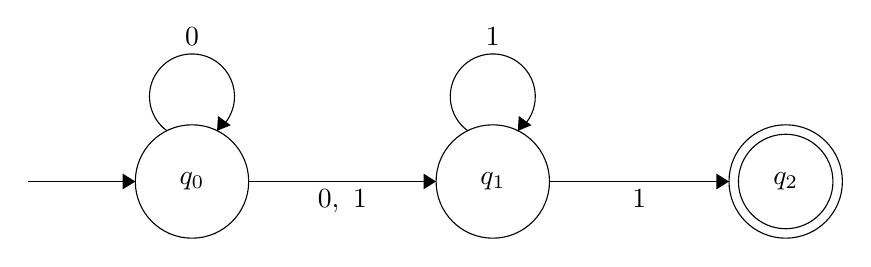
\begin{tikzpicture}[scale=0.2]
\tikzstyle{every node}+=[inner sep=0pt]
\draw [black] (10.6,-10.5) circle (3.6);
\draw (10.6,-10.5) node {$q_0$};
\draw [black] (29.7,-10.5) circle (3.6);
\draw (29.7,-10.5) node {$q_1$};
\draw [black] (48.3,-10.5) circle (3.6);
\draw (48.3,-10.5) node {$q_2$};
\draw [black] (48.3,-10.5) circle (3);
\draw [black] (14.2,-10.5) -- (26.1,-10.5);
\fill [black] (26.1,-10.5) -- (25.3,-10) -- (25.3,-11);
\draw (20.15,-11) node [below] {$0,\mbox{ }1$};
\draw [black] (33.3,-10.5) -- (44.7,-10.5);
\fill [black] (44.7,-10.5) -- (43.9,-10) -- (43.9,-11);
\draw (39,-11) node [below] {$1$};
\draw [black] (9.013,-7.284) arc (234:-54:2.7);
\draw (10.6,-1.9) node [above] {$0$};
\fill [black] (12.19,-7.28) -- (13.06,-6.93) -- (12.25,-6.34);
\draw [black] (28.113,-7.284) arc (234:-54:2.7);
\draw (29.7,-1.9) node [above] {$1$};
\fill [black] (31.29,-7.28) -- (32.16,-6.93) -- (31.35,-6.34);
\draw [black] (0.2,-10.5) -- (7,-10.5);
\fill [black] (7,-10.5) -- (6.2,-10) -- (6.2,-11);
\end{tikzpicture}
\end{center}

\vspace{5mm}

\noindent\textbf{Solution:}

\vspace{5mm}

\noindent NFA $\rightarrow$ DFA Conversion Table:

\vspace{1mm}

\noindent\begin{tabularx}{\textwidth} { 
  | >{\centering\arraybackslash}X 
  | >{\centering\arraybackslash}X 
  | >{\centering\arraybackslash}X | }
 \hline
 \rowcolor{lightgray} & 0 & 1 \\
\hline
$\{q_0\}$ & \textcolor{ForestGreen}{$\{q_0, q_1\}$} & \textcolor{ForestGreen}{$\{q_1\}$}  \\
\hline
$\{q_1\}$ & \textcolor{ForestGreen}{$\emptyset$} & \textcolor{ForestGreen}{$\{q_1, q_2\}$}  \\
\hline
$\{q_0, q_1\}$ & $\{q_0, q_1\}$ & $\{q_1, q_2\}$  \\
 \hline
\textcolor{BrickRed}{$\{q_1, q_2\} \in F$} & $\emptyset$ & $\{q_1, q_2\}$  \\
\hline
$\emptyset$ & $\emptyset$ & $\emptyset$  \\
\hline
\end{tabularx}

\vspace{5mm}

\noindent DFA Transition Graph:

\begin{center}
\begin{tikzpicture}[scale=0.2]
\tikzstyle{every node}+=[inner sep=0pt]
\draw [black] (13.1,-26) circle (3.7);
\draw (13.1,-26) node {$q_0$};
\draw [black] (34.2,-26) circle (3.7);
\draw (34.2,-26) node {$q_1$};
\draw [black] (57.5,-26) circle (3.7);
\draw (57.5,-26) node {$(q_1,\mbox{ }q_2)$};
\draw [black] (57.5,-26) circle (3.1);
\draw [black] (34.2,-10.7) circle (3.7);
\draw (34.2,-10.7) node {$(q_0,\mbox{ }q_1)$};
\draw [black] (45.3,-42.4) circle (3.7);
\draw (45.3,-42.4) node {$\emptyset$};
\draw [black] (16.8,-26) -- (30.5,-26);
\fill [black] (30.5,-26) -- (29.7,-25.5) -- (29.7,-26.5);
\draw (23.65,-26.5) node [below] {$1$};
\draw [black] (37.9,-26) -- (53.8,-26);
\fill [black] (53.8,-26) -- (53,-25.5) -- (53,-26.5);
\draw (45.85,-26.5) node [below] {$1$};
\draw [black] (60.197,-23.488) arc (160.69924:-127.30076:2.775);
\draw (66.24,-23) node [right] {$1$};
\fill [black] (61.13,-26.61) -- (61.72,-27.35) -- (62.05,-26.41);
\draw [black] (37.29,-12.73) -- (54.41,-23.97);
\fill [black] (54.41,-23.97) -- (54.01,-23.11) -- (53.46,-23.95);
\draw (44.85,-18.85) node [below] {$1$};
\draw [black] (33.02,-7.208) arc (226.40536:-61.59464:2.775);
\draw (35.61,-1.86) node [above] {$0$};
\fill [black] (36.25,-7.64) -- (37.17,-7.4) -- (36.44,-6.72);
\draw [black] (16.1,-23.83) -- (31.2,-12.87);
\fill [black] (31.2,-12.87) -- (30.26,-12.94) -- (30.85,-13.75);
\draw (24.65,-18.85) node [below] {$0$};
\draw [black] (0.2,-26) -- (9.4,-26);
\fill [black] (9.4,-26) -- (8.6,-25.5) -- (8.6,-26.5);
\draw [black] (48.951,-41.898) arc (125.56505:-162.43495:2.775);
\draw (53.96,-45.74) node [right] {$0,\mbox{ }1$};
\fill [black] (47.92,-44.99) -- (47.98,-45.93) -- (48.79,-45.35);
\draw [black] (36.27,-29.06) -- (43.23,-39.34);
\fill [black] (43.23,-39.34) -- (43.19,-38.39) -- (42.36,-38.95);
\draw (39.14,-35.54) node [left] {$0$};
\draw [black] (55.29,-28.97) -- (47.51,-39.43);
\fill [black] (47.51,-39.43) -- (48.39,-39.09) -- (47.58,-38.49);
\draw (50.82,-32.81) node [left] {$0$};
\end{tikzpicture}
\end{center}

\newpage

\section*{Problem 3: [5 points]}

For any string $\omega$ (over some alphabet $\sum$), let $\tilde{\omega}$ denote the reverse of $\omega$, i.e., writing $\omega$ from right to left. For example, if $\omega = bbbaba$ then $\tilde{\omega} = ababbb$. Furthermore, for any language $L$, let

\vspace{5mm}

$\tilde{L} = \{\tilde{\omega}|\omega \in L\},$

\vspace{5mm}

\noindent i.e., $\tilde{L}$ is the set of all strings that are the reverse of some string in $L$.

\vspace{5mm}

\noindent Prove that if $L$ is a regular language, then $\tilde{L}$ is also a regular language.

\vspace{5mm}

\noindent \textbf{Hint:} There might be multiple ways to prove this. I personally think the easiest way is to construct a regular expression that represents $\tilde{L}$.

\vspace{5mm}

\noindent\textbf{Solution:}

\vspace{5mm}

\noindent let $L$ be a regular language over the alphabet $\sum = \{a, b\}$ which can be represented by the regular expression $r = a^*b$ or all strings that consist of zero or more a's followed by a b. Some example strings in $L$ are: 
\begin{itemize}
	\item $b$
	\item $ab$
	\item $aab$
	\item $aaab$
	\item and so on...
\end{itemize}

\noindent We now want to find $\tilde{L}$, or the set of strings that are the reverse of every string in $L$. So let's reverse the regular expression $r$ into $\tilde{r} = \tilde{(ba^*)} = ba^*$, and now $\tilde{r} = ba^*$ represents the reverse $\tilde{L}$. This represents all strings that start with a b that are followed by zero or more a's. Some example strings in $\tilde{L}$ are:
\begin{itemize}
	\item $b$
	\item $ba$
	\item $ba$
	\item $baaa$
	\item and so on...
\end{itemize}

\noindent To verify this, let's take some example strings from $L$ and reverse them and make sure that they are in $\tilde{L}$.
\begin{itemize}
	\item If $\omega = b \in L$, then $\tilde{\omega} = b \in \tilde{L}$
	\item If $\omega = ab \in L$, then $\tilde{\omega} = ba \in \tilde{L}$
	\item If $\omega = aab \in L$, then $\tilde{\omega} = baa \in \tilde{L}$
\end{itemize}

\noindent All the reversed strings are in $\tilde{L}$ and is accurately represented by the regular expression $\tilde{r} = ba^*$ which proves that the languages $L$ and $\tilde{L}$ are indeed regular.

\noindent QED

\end{document}